\documentclass{standalone}
\usepackage{tikz}
\usetikzlibrary{patterns, positioning}

\begin{document}
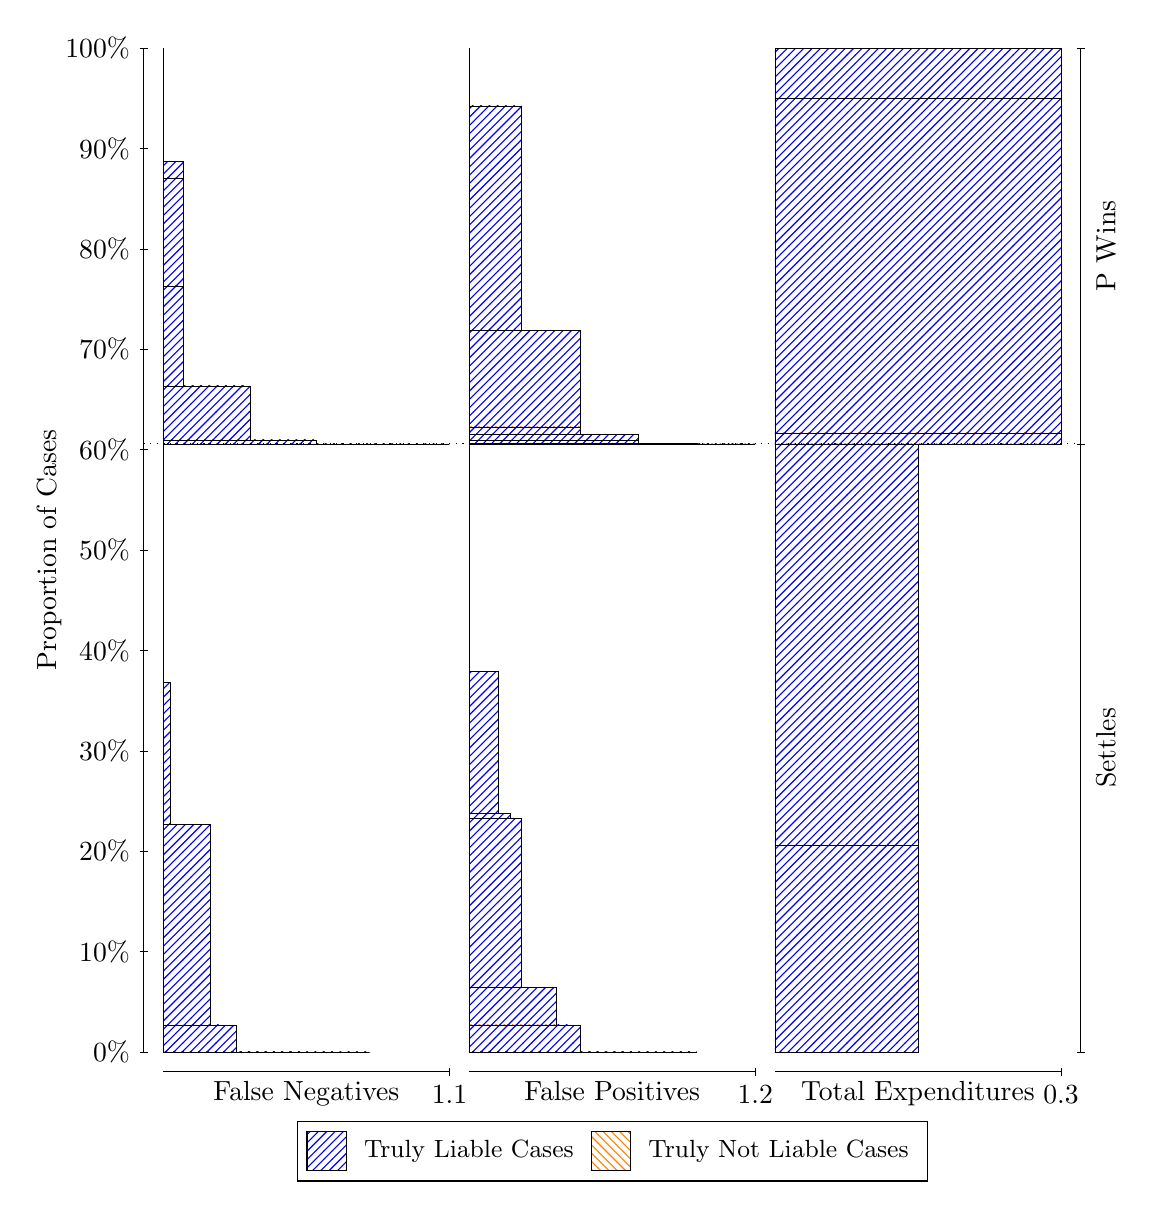
\begin{tikzpicture}
\draw[black, very thin] (1.5,1.75) -- (1.5,14.5);
\node[rotate=90, anchor=center] at (0.3, 8.125) {Proportion of Cases};
\draw[black, very thin] (1.45,1.75) -- (1.55,1.75);
\node[anchor=east] at (1.45, 1.75) {0\%};
\draw[black, very thin] (1.45,3.025) -- (1.55,3.025);
\node[anchor=east] at (1.45, 3.025) {10\%};
\draw[black, very thin] (1.45,4.3) -- (1.55,4.3);
\node[anchor=east] at (1.45, 4.3) {20\%};
\draw[black, very thin] (1.45,5.575) -- (1.55,5.575);
\node[anchor=east] at (1.45, 5.575) {30\%};
\draw[black, very thin] (1.45,6.85) -- (1.55,6.85);
\node[anchor=east] at (1.45, 6.85) {40\%};
\draw[black, very thin] (1.45,8.125) -- (1.55,8.125);
\node[anchor=east] at (1.45, 8.125) {50\%};
\draw[black, very thin] (1.45,9.4) -- (1.55,9.4);
\node[anchor=east] at (1.45, 9.4) {60\%};
\draw[black, very thin] (1.45,10.675) -- (1.55,10.675);
\node[anchor=east] at (1.45, 10.675) {70\%};
\draw[black, very thin] (1.45,11.95) -- (1.55,11.95);
\node[anchor=east] at (1.45, 11.95) {80\%};
\draw[black, very thin] (1.45,13.225) -- (1.55,13.225);
\node[anchor=east] at (1.45, 13.225) {90\%};
\draw[black, very thin] (1.45,14.5) -- (1.55,14.5);
\node[anchor=east] at (1.45, 14.5) {100\%};

\draw[black, very thin] (13.4,1.75) -- (13.4,14.5);
\draw[black, very thin] (13.35,1.75) -- (13.45,1.75);
\node[anchor=west] at (13.35, 1.75) {};
\draw[black, very thin] (13.35,9.4734) -- (13.45,9.4734);
\node[anchor=west] at (13.35, 9.4734) {};
\draw[black, very thin] (13.35,14.5) -- (13.45,14.5);
\node[anchor=west] at (13.35, 14.5) {};

\draw[black, very thin, pattern color=blue, pattern=north east lines] (1.75,1.75) rectangle (4.3694,1.75);
\draw[black, very thin, pattern color=blue, pattern=north east lines] (1.75,1.75) rectangle (3.5244,1.7505);
\draw[black, very thin, pattern color=blue, pattern=north east lines] (1.75,1.7505) rectangle (3.3554,1.7505);
\draw[black, very thin, pattern color=blue, pattern=north east lines] (1.75,1.7505) rectangle (2.6795,2.0904);
\draw[black, very thin, pattern color=blue, pattern=north east lines] (1.75,2.0904) rectangle (2.5105,2.0933);
\draw[black, very thin, pattern color=blue, pattern=north east lines] (1.75,2.0933) rectangle (2.3415,4.6391);
\draw[black, very thin, pattern color=blue, pattern=north east lines] (1.75,4.6391) rectangle (1.8345,6.4433);
\draw[black, very thin, pattern color=orange, pattern=north west lines] (1.75,6.4433) rectangle (1.75,6.4433);
\draw[black, very thin, pattern color=blue, pattern=north east lines] (1.75,6.4433) rectangle (1.75,9.4734);
\draw[black, very thin, pattern color=blue, pattern=north east lines] (1.75,9.4734) rectangle (5.3833,9.4734);
\draw[black, very thin, pattern color=blue, pattern=north east lines] (1.75,9.4734) rectangle (4.5384,9.4736);
\draw[black, very thin, pattern color=blue, pattern=north east lines] (1.75,9.4736) rectangle (3.6934,9.5233);
\draw[black, very thin, pattern color=blue, pattern=north east lines] (1.75,9.5233) rectangle (2.8484,10.208);
\draw[black, very thin, pattern color=blue, pattern=north east lines] (1.75,10.208) rectangle (2.8484,10.209);
\draw[black, very thin, pattern color=blue, pattern=north east lines] (1.75,10.209) rectangle (2.0035,11.48);
\draw[black, very thin, pattern color=blue, pattern=north east lines] (1.75,11.48) rectangle (2.0035,12.851);
\draw[black, very thin, pattern color=blue, pattern=north east lines] (1.75,12.851) rectangle (2.0035,13.058);
\draw[black, very thin, pattern color=orange, pattern=north west lines] (1.75,13.058) rectangle (1.75,13.058);
\draw[black, very thin, pattern color=blue, pattern=north east lines] (1.75,13.058) rectangle (1.75,14.5);
\draw[black, very thin, pattern color=orange, pattern=north west lines] (5.6333,1.75) rectangle (8.5252,1.75);
\draw[black, very thin, pattern color=blue, pattern=north east lines] (5.6333,1.75) rectangle (8.5252,1.75);
\draw[black, very thin, pattern color=blue, pattern=north east lines] (5.6333,1.75) rectangle (7.7837,1.7505);
\draw[black, very thin, pattern color=orange, pattern=north west lines] (5.6333,1.7505) rectangle (7.6354,1.7505);
\draw[black, very thin, pattern color=blue, pattern=north east lines] (5.6333,1.7505) rectangle (7.6354,1.7505);
\draw[black, very thin, pattern color=blue, pattern=north east lines] (5.6333,1.7505) rectangle (7.0422,2.0909);
\draw[black, very thin, pattern color=blue, pattern=north east lines] (5.6333,2.0909) rectangle (6.8939,2.0938);
\draw[black, very thin, pattern color=orange, pattern=north west lines] (5.6333,2.0938) rectangle (6.7456,2.0938);
\draw[black, very thin, pattern color=blue, pattern=north east lines] (5.6333,2.0938) rectangle (6.7456,2.5739);
\draw[black, very thin, pattern color=blue, pattern=north east lines] (5.6333,2.5739) rectangle (6.3007,4.7159);
\draw[black, very thin, pattern color=blue, pattern=north east lines] (5.6333,4.7159) rectangle (6.1524,4.7801);
\draw[black, very thin, pattern color=blue, pattern=north east lines] (5.6333,4.7801) rectangle (6.0041,6.5843);
\draw[black, very thin, pattern color=blue, pattern=north east lines] (5.6333,6.5843) rectangle (5.6333,9.4734);
\draw[black, very thin, pattern color=orange, pattern=north west lines] (5.6333,9.4734) rectangle (9.2667,9.4734);
\draw[black, very thin, pattern color=blue, pattern=north east lines] (5.6333,9.4734) rectangle (9.2667,9.4734);
\draw[black, very thin, pattern color=blue, pattern=north east lines] (5.6333,9.4734) rectangle (8.5252,9.4737);
\draw[black, very thin, pattern color=orange, pattern=north west lines] (5.6333,9.4737) rectangle (8.5252,9.4737);
\draw[black, very thin, pattern color=blue, pattern=north east lines] (5.6333,9.4737) rectangle (8.5252,9.4749);
\draw[black, very thin, pattern color=blue, pattern=north east lines] (5.6333,9.4749) rectangle (7.7837,9.5152);
\draw[black, very thin, pattern color=orange, pattern=north west lines] (5.6333,9.5152) rectangle (7.7837,9.5152);
\draw[black, very thin, pattern color=blue, pattern=north east lines] (5.6333,9.5152) rectangle (7.7837,9.594);
\draw[black, very thin, pattern color=blue, pattern=north east lines] (5.6333,9.594) rectangle (7.0422,9.6891);
\draw[black, very thin, pattern color=orange, pattern=north west lines] (5.6333,9.6891) rectangle (7.0422,9.6891);
\draw[black, very thin, pattern color=blue, pattern=north east lines] (5.6333,9.6891) rectangle (7.0422,10.915);
\draw[black, very thin, pattern color=blue, pattern=north east lines] (5.6333,10.915) rectangle (6.3007,10.918);
\draw[black, very thin, pattern color=orange, pattern=north west lines] (5.6333,10.918) rectangle (6.3007,10.918);
\draw[black, very thin, pattern color=blue, pattern=north east lines] (5.6333,10.918) rectangle (6.3007,13.764);
\draw[black, very thin, pattern color=blue, pattern=north east lines] (5.6333,13.764) rectangle (5.6333,14.5);
\draw[black, very thin, pattern color=orange, pattern=north west lines] (9.5167,1.75) rectangle (11.333,1.75);
\draw[black, very thin, pattern color=blue, pattern=north east lines] (9.5167,1.75) rectangle (11.333,4.3746);
\draw[black, very thin, pattern color=orange, pattern=north west lines] (9.5167,4.3746) rectangle (11.333,4.3746);
\draw[black, very thin, pattern color=blue, pattern=north east lines] (9.5167,4.3746) rectangle (11.333,9.4734);
\draw[black, very thin, pattern color=orange, pattern=north west lines] (9.5167,9.4734) rectangle (13.15,9.4734);
\draw[black, very thin, pattern color=blue, pattern=north east lines] (9.5167,9.4734) rectangle (13.15,9.6119);
\draw[black, very thin, pattern color=orange, pattern=north west lines] (9.5167,9.6119) rectangle (13.15,9.6119);
\draw[black, very thin, pattern color=blue, pattern=north east lines] (9.5167,9.6119) rectangle (13.15,13.86);
\draw[black, very thin, pattern color=orange, pattern=north west lines] (9.5167,13.86) rectangle (13.15,13.86);
\draw[black, very thin, pattern color=blue, pattern=north east lines] (9.5167,13.86) rectangle (13.15,14.5);
\draw[black, dotted] (1.5,9.4734) -- (13.4,9.4734);
\draw[black, very thin] (1.75,1.5) -- (5.3833,1.5);
\node[anchor=north] at (3.5667, 1.5) {False Negatives};
\draw[black, very thin] (5.3833,1.45) -- (5.3833,1.55);
\node[anchor=north] at (5.3833, 1.45) {1.1};

\draw[black, very thin] (5.6333,1.5) -- (9.2667,1.5);
\node[anchor=north] at (7.45, 1.5) {False Positives};
\draw[black, very thin] (9.2667,1.45) -- (9.2667,1.55);
\node[anchor=north] at (9.2667, 1.45) {1.2};

\draw[black, very thin] (9.5167,1.5) -- (13.15,1.5);
\node[anchor=north] at (11.333, 1.5) {Total Expenditures};
\draw[black, very thin] (13.15,1.45) -- (13.15,1.55);
\node[anchor=north] at (13.15, 1.45) {0.3};

\node[black, centered, rotate=90] at (13.72, 5.6117) {Settles};
\node[black, centered, rotate=90] at (13.72, 11.987) {P Wins};

\draw (7.449999999999999,1.5) node[draw=none] (baseCoordinate) {};
\begin{scope}[align=center]
        \matrix[scale=0.5, draw=black, below=0.5cm of baseCoordinate, nodes={draw}, column sep=0.1cm]{
            \node[rectangle, draw, minimum width=0.5cm, minimum height=0.5cm, pattern=north east lines, pattern color=blue] {}; &
            \node[draw=none, font=\small] (B) {Truly Liable Cases}; &
            \node[rectangle, draw, minimum width=0.5cm, minimum height=0.5cm, pattern=north west lines, pattern color=orange] {}; &
            \node[draw=none, font=\small] (B) {Truly Not Liable Cases}; \\
            };
\end{scope}

\end{tikzpicture}
\end{document}